% ============================================================
%  PRÉSENTATION FINALE — Projet PF22 — Approche Multi-Fidélité
%  Auteur : Ivann Vasic — UTBM — Module PF22 — Soutenance 26 juin 2026
%  Thème : identité du rapport final (bleu UTBM + logo)
%  Durée cible : ~10 minutes (public connaisseur du domaine DL)
% ============================================================
\documentclass[aspectratio=169, 11pt]{beamer}

\usepackage[utf8]{inputenc}
\usepackage[T1]{fontenc}
\usepackage[french]{babel}
\usepackage{lmodern}
\usepackage{helvet}
\renewcommand{\familydefault}{\sfdefault}
\usepackage{microtype}
\usepackage{graphicx}
\usepackage{booktabs}
\usepackage{tabularx}
\usepackage{array}
\usepackage{colortbl}
\usepackage{amsmath}
\usepackage{amssymb}
\usepackage{xcolor}
\usepackage{tcolorbox}
\tcbuselibrary{skins}

% ============================================================
%  PALETTE (identité UTBM, cohérente avec le rapport)
% ============================================================
\definecolor{utbmblue}{HTML}{1F7EC2}
\definecolor{utbmdark}{HTML}{17597F}
\definecolor{ink}{HTML}{1C2434}
\definecolor{muted}{HTML}{6E7A8E}
\definecolor{rule}{HTML}{DEE3EB}
\definecolor{headerbg}{HTML}{EAF2F9}
\definecolor{success}{HTML}{2E8B57}
\definecolor{warn}{HTML}{C77A22}
\definecolor{danger}{HTML}{B03A3A}

% ============================================================
%  THÈME
% ============================================================
\usetheme{default}
\usecolortheme{default}
\setbeamertemplate{navigation symbols}{}
\setbeamertemplate{frametitle continuation}{}

\setbeamercolor{background canvas}{bg=white}
\setbeamercolor{normal text}{fg=ink}
\setbeamercolor{frametitle}{fg=utbmdark}
\setbeamerfont{frametitle}{series=\bfseries, size=\large}
\setbeamercolor{itemize item}{fg=utbmblue}
\setbeamercolor{itemize subitem}{fg=muted}
\setbeamertemplate{itemize item}{\color{utbmblue}\small$\blacktriangleright$}
\setbeamertemplate{itemize subitem}{\color{muted}\scriptsize$-$}
\setbeamercolor{block title}{fg=white, bg=utbmblue}
\setbeamercolor{block body}{fg=ink, bg=headerbg}
\setlength{\parskip}{2pt}

% --- Titre de frame : indenté + filet bleu ---
\setbeamertemplate{frametitle}{%
  \nointerlineskip%
  \vspace{0.32cm}%
  \hspace{0.6cm}{\usebeamerfont{frametitle}\color{utbmdark}\insertframetitle}%
  \par\vspace{2pt}%
  \hspace{0.6cm}{\color{utbmblue}\rule{0.90\paperwidth}{1.3pt}}%
  \par\vspace{2pt}%
}

% --- Pied de page : filet fin + infos ---
\setbeamertemplate{footline}{%
  \leavevmode%
  \hbox{%
    \begin{beamercolorbox}[wd=\paperwidth, ht=2.4ex, dp=1.1ex]{normal text}%
      \hspace{0.65cm}{\color{muted}\scriptsize PF22 $\cdot$ Approche Multi-Fidélité}%
      \hfill{\color{muted}\scriptsize Ivann Vasic \;\textbar\;}%
      \,{\color{utbmblue}\scriptsize\bfseries\insertframenumber\,/\,\inserttotalframenumber}%
      \hspace{0.65cm}%
    \end{beamercolorbox}}%
  \vspace{1.5pt}%
}

% ============================================================
%  BOÎTES UTILITAIRES
% ============================================================
% Carte à bandeau-titre (stratégies, notions)
\newtcolorbox{card}[1][]{
  enhanced, colback=utbmblue!4, colframe=utbmblue,
  boxrule=0.5pt, leftrule=2pt, arc=2pt,
  fonttitle=\bfseries\footnotesize, coltitle=white, colbacktitle=utbmblue,
  title={#1}, left=5pt, right=5pt, top=3pt, bottom=3pt,
  fontupper=\footnotesize
}
% Encadré "message clé"
\newtcolorbox{key}{
  enhanced, colback=gray!5, colframe=utbmdark,
  boxrule=0.4pt, leftrule=3pt, arc=2pt,
  left=7pt, right=7pt, top=4pt, bottom=4pt, fontupper=\small
}

% Petits raccourcis
\newcommand{\hf}{\textbf{\color{hfcolor}HF}}
\definecolor{hfcolor}{HTML}{1F518C}
\newcommand{\HF}{\textbf{HF}}
\newcommand{\BF}{\textbf{BF}}
\newcommand{\res}[2]{#1\,{\scriptsize$\pm$#2}}

% ============================================================
%  DOCUMENT
% ============================================================
\begin{document}

% -------------------- TITRE --------------------
\begin{frame}[plain]
  \centering
  \vspace{0.35cm}
  
\includegraphics[width=4.1cm]{figures/utbm.png}\\[0.55cm]

  {\small\color{utbmdark}\textbf{UNIVERSITÉ DE TECHNOLOGIE DE BELFORT-MONTBÉLIARD}}\\[0.2em]
  {\scriptsize\color{muted}Module \textbf{PF22} — Apprentissage profond}\\[0.8cm]

  {\color{utbmblue}\rule{0.78\paperwidth}{1.6pt}}\\[0.32em]
  {\LARGE\bfseries\color{ink}Réduction des Coûts d'Apprentissage}\\[0.12em]
  {\LARGE\bfseries\color{utbmblue}par Approche Multi-Fidélité}\\[0.30em]
  {\color{utbmblue}\rule{0.78\paperwidth}{1.6pt}}\\[0.6cm]

  {\small\color{muted}Combiner \emph{peu} d'images Haute Fidélité (coûteuses) et
  \emph{beaucoup} d'images Basse Fidélité (bon marché)}\\[0.9cm]

  {\color{ink}\large\textbf{Ivann Vasic}}\\[0.18em]
  {\scriptsize\color{muted}Soutenance — 26 juin 2026 \quad\textbullet\quad UTBM}
\end{frame}

% -------------------- CONTEXTE --------------------
\begin{frame}{Contexte \& problématique}
  \begin{columns}[T]
    \begin{column}{0.56\textwidth}
      \textbf{Le constat}
      \begin{itemize}
        \item La performance d'un réseau dépend de la \textbf{quantité} \emph{et} de la \textbf{qualité} des données.
        \item Données \textbf{Haute Fidélité} : haute résolution, experts, capteurs chers $\rightarrow$ \textcolor{danger}{rares et coûteuses}.
        \item Données \textbf{Basse Fidélité} : dégradées, web, capteurs bas de gamme $\rightarrow$ \textcolor{success}{abondantes et bon marché}.
      \end{itemize}
      \vspace{0.3em}
      \textbf{L'idée : l'apprentissage multi-fidélité}
      \begin{itemize}
        \item Mélanger un \emph{petit} volume HF avec un \emph{grand} volume BF.
        \item La vraie question n'est plus « quelle précision ? » mais
        « \textbf{quelle précision pour quel budget ?} ».
      \end{itemize}
    \end{column}
    \begin{column}{0.42\textwidth}
      \begin{key}
        \textbf{Problématique.} Comment exploiter beaucoup de données BF bon marché
        pour \textbf{maximiser la précision sur le domaine HF}, tout en
        \textbf{minimisant le coût d'acquisition} ?
      \end{key}
      \vspace{0.5em}
      \begin{center}
        \footnotesize\color{utbmdark}\textbf{Etude réalisé sur de la classification d'images}\\[2pt]
      \end{center}
    \end{column}
  \end{columns}
\end{frame}

% -------------------- HF vs BF (exemples) --------------------
\begin{frame}{Concrètement : Haute Fidélité vs Basse Fidélité}
  \begin{columns}[c]
    \begin{column}{0.62\textwidth}
      \centering
      \setlength{\tabcolsep}{3pt}\renewcommand{\arraystretch}{1.0}
      \begin{tabular}{c ccc}
         & {\scriptsize\textbf{Animals-10}} & {\scriptsize\textbf{Imagewoof}} & {\scriptsize\textbf{Intel}}\\[2pt]
        \rotatebox{90}{\scriptsize\ \,\textbf{HF}} &
          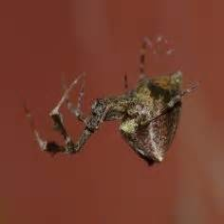
\includegraphics[height=2.25cm]{figures/sample_Animals-10_HF.png} &
          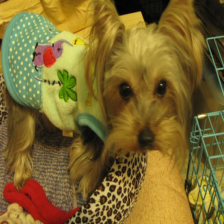
\includegraphics[height=2.25cm]{figures/sample_Imagewoof_HF.png} &
          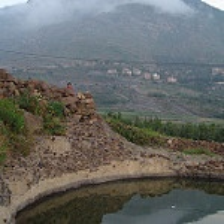
\includegraphics[height=2.25cm]{figures/sample_Intel_HF.png}\\[3pt]
        \rotatebox{90}{\scriptsize\ \,\textbf{BF}} &
          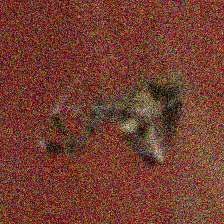
\includegraphics[height=2.25cm]{figures/sample_Animals-10_BF.png} &
          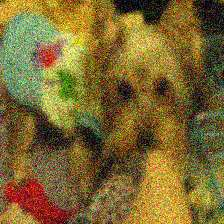
\includegraphics[height=2.25cm]{figures/sample_Imagewoof_BF.png} &
          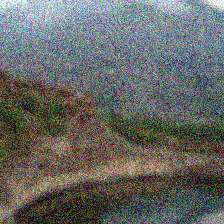
\includegraphics[height=2.25cm]{figures/sample_Intel_BF.png}\\
      \end{tabular}
    \end{column}
    \begin{column}{0.36\textwidth}
      \begin{card}[Dégradation BF canonique]
        Sous-échantillonnage \textbf{224\,$\rightarrow$\,64\,px}\\
        $+$ bruit gaussien \textbf{$\sigma=0{,}15$}\\
        $+$ compression \textbf{JPEG $q60$}
      \end{card}
      \vspace{0.4em}
      \footnotesize
      Appliquée \textbf{à la volée} et \textbf{déterministe par image}
      (train BF $=$ test BF, pas de décalage parasite).
    \end{column}
  \end{columns}
  \vspace{0.3em}
  \begin{center}\scriptsize\color{muted}
    3 datasets de natures différentes (animaux, races fine-grained, scènes) pour valider la généralité.
  \end{center}
\end{frame}

% -------------------- PIPELINE & PROTOCOLE --------------------
\begin{frame}{Protocole expérimental}
  \begin{columns}[T]
    \begin{column}{0.5\textwidth}
      \textbf{Découpage des données}
      \begin{itemize}
        \item Test \textbf{10\,\%} (100\,\% HF) ; Train \textbf{90\,\%}.
        \item Train découpé en \textbf{10\,\% HF} $+$ \textbf{90\,\% BF}.
      \end{itemize}
      \vspace{0.2em}
      \textbf{Évaluation croisée}
      \begin{itemize}
        \item 3 jeux de test : \textbf{HF}, \textbf{BF}, \textbf{Mixte}.
        \item Critère prioritaire : \textbf{Test HF}.
      \end{itemize}
    \end{column}
    \begin{column}{0.5\textwidth}
      \textbf{Rigueur \& reproductibilité}
      \begin{itemize}
        \item Modèle : \textbf{ResNet-18 \emph{from scratch}}.
        \item \textbf{3 datasets} $\times$ \textbf{3 seeds} $\rightarrow$ moyenne $\pm$ écart-type.
        \item Dégradation centralisée \& déterministe.
        \item Calcul sur \textbf{serveur GPU V100S}.
      \end{itemize}
      \vspace{0.4em}
      \begin{key}
        \footnotesize Tout résultat est reporté en \textbf{moyenne $\pm$ écart-type}
        sur 3 seeds $\rightarrow$ conclusions robustes au hasard d'initialisation.
      \end{key}
    \end{column}
  \end{columns}
\end{frame}

% -------------------- MODÈLE DE COÛT --------------------
\begin{frame}{Modéliser le coût}
  \begin{columns}[T]
    \begin{column}{0.54\textwidth}
      \textbf{Trois métriques distinctes}
      \begin{itemize}
        \item \textbf{Coût donnée} : acquisition, payé \emph{une fois}.
        \item \textbf{Coût calcul} : images vues à l'entraînement.
        \item \textbf{Coût total} : calcul pondéré par le coût donnée.
      \end{itemize}
      \vspace{0.3em}
      \textbf{Formule du coût unitaire (résolution d)}
      \[
        \footnotesize
        C(d) = C_{\min} + (C_{\mathrm{HF}}-C_{\min})\Big(\tfrac{d}{224}\Big)^{2}
      \]
      \footnotesize Calibration : \textbf{HF $=$ 10}, \textbf{BF (64\,px) $=$ 1}
      $\Rightarrow$ ratio de coût \textbf{10\,:\,1}.
    \end{column}
    \begin{column}{0.44\textwidth}
      \begin{card}[Exemple — Animals-10]
        Pool d'entraînement :\\
        2\,352 HF \;+\; 21\,213 BF
        \[
          \scriptsize
          \underbrace{2\,352\times 10}_{\text{HF}} + \underbrace{21\,213\times 1}_{\text{BF}}
          = \textbf{44\,733 CA}
        \]
        \scriptsize C'est le \textbf{coût donnée} commun à toute méthode utilisant le pool complet.
      \end{card}
      \vspace{0.3em}
      \begin{center}\scriptsize\color{muted}
        Les méthodes se départagent alors sur le \textbf{coût total} (passages sur le HF coûteux).
      \end{center}
    \end{column}
  \end{columns}
\end{frame}

% -------------------- BASELINES --------------------
\begin{frame}{Modèles de référence (Baselines)}
  \footnotesize
  \setlength{\tabcolsep}{5pt}\renewcommand{\arraystretch}{1.25}
  \begin{center}
  \begin{tabular}{@{}lccc@{}}
    \toprule
    \rowcolor{headerbg}
    \textbf{Baseline (Animals-10)} & \textbf{Test HF} & \textbf{Test BF} & \textbf{Coût donnée}\\
    \midrule
    BL\,1 — Premium (HF seul)   & \res{54,3}{2,2} & \res{27,8}{0,8} & 23\,520\\
    BL\,2 — Low-Cost (BF seul)  & \res{61,3}{6,3} & \res{71,0}{1,5} & 21\,213\\
    BL\,3 — Mixte (borne haute) & \res{74,0}{3,0} & \res{72,9}{1,1} & 44\,733\\
    \bottomrule
  \end{tabular}
  \end{center}
  \vspace{0.2em}
  \begin{columns}[T]
    \begin{column}{0.5\textwidth}
      \begin{card}[Effondrement face au bruit]
        BL\,1 (HF seul) : \textbf{54,3\,\% $\rightarrow$ 27,8\,\%} sur BF.
        Le \emph{domain shift}.
      \end{card}
    \end{column}
    \begin{column}{0.5\textwidth}
      \begin{card}[Paradoxe de la quantité]
        BL\,2 (BF seul) bat BL\,1 \textbf{même sur HF}
        (61,3 vs 54,3\,\%) pour un coût \emph{inférieur}.
      \end{card}
    \end{column}
  \end{columns}
  \vspace{0.2em}
  \begin{center}\scriptsize\color{muted}
    BL\,3 (Mixte) $=$ borne supérieure à atteindre… mais coûteuse. \textbf{Objectif : l'égaler à moindre coût.}
  \end{center}
\end{frame}

% -------------------- LES 4 STRATÉGIES --------------------
\begin{frame}{Quatre stratégies multi-fidélité (objectif HF)}
  \begin{columns}[t]
    \begin{column}{0.49\textwidth}
      \begin{card}[S1 · Transfer Learning séquentiel]
        Pré-entraînement sur le volume \BF, puis \textbf{fine-tuning} sur le sous-ensemble \HF.
        \emph{(BF $\rightarrow$ HF)}
      \end{card}
      \vspace{4pt}
      \begin{card}[S3 · Curriculum Learning]
        Un seul entraînement où la \textbf{proportion de HF augmente par paliers}
        (0\,\% $\rightarrow$ 100\,\%). Transition douce.
      \end{card}
    \end{column}
    \begin{column}{0.49\textwidth}
      \begin{card}[S2 · Co-training pondéré]
        HF \emph{et} BF dans \textbf{chaque batch}, avec une \textbf{pondération}
        de la perte favorisant le HF.
      \end{card}
      \vspace{4pt}
      \begin{card}[S4 · EWC (Elastic Weight Consolidation)]
        Transfert séquentiel $+$ \textbf{pénalité de Fisher} protégeant les poids
        importants pour le BF (anti-oubli).
      \end{card}
    \end{column}
  \end{columns}
  \vspace{0.3em}
  \begin{center}\scriptsize\color{muted}
    Chaque stratégie est aussi déclinée en version \textbf{optimisée par Optuna}.
  \end{center}
\end{frame}


% -------------------- RÉSULTATS : TABLEAU DE SYNTHÈSE --------------------
\begin{frame}{Résultats — synthèse globale (BL\,3 + 4 stratégies)}
  \centering
  \vspace*{-0.45cm}
  \scriptsize
  \setlength{\tabcolsep}{4pt}\renewcommand{\arraystretch}{0.92}
  \begin{tabularx}{\linewidth}{@{}l *{5}{>{\centering\arraybackslash}X}@{}}
    \toprule
    \rowcolor{headerbg}
    \textbf{Modèle} & \textbf{HF} & \textbf{BF} & \textbf{Mixte} & \textbf{Coût donnée} & \textbf{Coût total}\\
    \midrule
    \multicolumn{6}{l}{\textit{\textbf{Animals-10}}}\\
    BL\,3 (Mixte) & \res{74,0}{3,0} & \res{72,9}{1,1} & \res{73,4}{2,0} & 44\,733 & 894\,660\\
    Stratégie 1   & \res{77,7}{0,6} & \res{68,3}{0,5} & \res{73,0}{0,3} & 44\,733 & 400\,230\\
    Stratégie 2   & \res{63,8}{5,2} & \res{61,0}{4,2} & \res{62,4}{4,7} & 44\,733 & 486\,720\\
    Stratégie 3   & \res{76,5}{0,2} & \res{73,1}{0,1} & \res{74,8}{0,1} & 44\,733 & 421\,265\\
    \textbf{Stratégie 4 (EWC)} & \textbf{\res{78,0}{0,3}} & \res{68,8}{0,7} & \res{73,4}{0,4} & 44\,733 & \textbf{400\,230}\\
    \midrule
    \multicolumn{6}{l}{\textit{\textbf{Imagewoof}}}\\
    BL\,3 (Mixte) & \res{50,3}{2,5} & \res{48,8}{2,3} & \res{49,6}{2,4} & 17\,116 & 342\,320\\
    Stratégie 1   & \res{51,0}{1,6} & \res{44,7}{1,3} & \res{47,9}{1,5} & 17\,116 & 153\,160\\
    Stratégie 2   & \res{37,5}{0,8} & \res{37,4}{0,3} & \res{37,5}{0,2} & 17\,116 & 183\,040\\
    Stratégie 3   & \res{47,5}{1,4} & \res{46,1}{1,1} & \res{46,8}{1,2} & 17\,116 & 158\,880\\
    \textbf{Stratégie 4 (EWC)} & \textbf{\res{53,3}{0,7}} & \res{46,8}{0,6} & \res{50,0}{0,6} & 17\,116 & \textbf{153\,160}\\
    \midrule
    \multicolumn{6}{l}{\textit{\textbf{Intel}}}\\
    BL\,3 (Mixte) & \res{82,8}{1,2} & \res{82,1}{1,2} & \res{82,5}{1,2} & 26\,652 & 533\,040\\
    \textbf{Stratégie 1}   & \textbf{\res{86,1}{0,4}} & \res{79,1}{1,4} & \res{82,6}{0,7} & 26\,652 & \textbf{238\,420}\\
    Stratégie 2   & \res{82,0}{1,0} & \res{79,8}{0,9} & \res{80,9}{0,9} & 26\,652 & 291\,200\\
    Stratégie 3   & \res{84,6}{1,0} & \res{82,6}{1,5} & \res{83,6}{1,2} & 26\,652 & 250\,880\\
    Stratégie 4 (EWC) & \res{85,8}{0,4} & \res{80,0}{0,9} & \res{82,9}{0,6} & 26\,652 & 238\,420\\
    \bottomrule
  \end{tabularx}

  \vspace{0.25em}
  {\tiny\color{muted} En gras : meilleur \textbf{Test HF} par dataset. Coût \emph{donnée} identique (pool complet) ; les stratégies se départagent sur le \textbf{coût total}.}
\end{frame}

% -------------------- OPTUNA --------------------
\begin{frame}{Optimisation des hyperparamètres (Optuna)}
  \begin{columns}[T]
    \begin{column}{0.5\textwidth}
      \textbf{Méthode}
      \begin{itemize}
        \item Recherche bayésienne (TPE), \textbf{20 essais} par stratégie $\times$ dataset.
        \item Objectif : précision de validation HF.
      \end{itemize}
      \vspace{0.3em}
      \textbf{Ce qu'on apprend}
      \begin{itemize}
        \item Gros gains sur les stratégies \textbf{instables} :
        Co-training \textcolor{success}{$+9{,}4$ pts} (Animals),
        Curriculum \textcolor{success}{$+5{,}3$ pts} (Imagewoof).
      \end{itemize}
    \end{column}
    \begin{column}{0.5\textwidth}
      \begin{card}[Limite observée]
        Peu — voire pas — de gain sur les stratégies \textbf{déjà fortes et stables}
        (S1, EWC) : EWC se dégrade même ($\lambda$ trop relâché),
        signe d'un léger sur-ajustement à la validation (budget de 20 essais).
      \end{card}
      \vspace{0.4em}
      \begin{center}\scriptsize\color{muted}
        Piste : optimisation \textbf{multi-objectif} (précision \emph{et} coût) avec plus d'essais.
      \end{center}
    \end{column}
  \end{columns}
\end{frame}

% -------------------- RÉSULTATS : PRÉCISION HF --------------------
\begin{frame}{Résultats — précision HF par modèle}
  \centering
  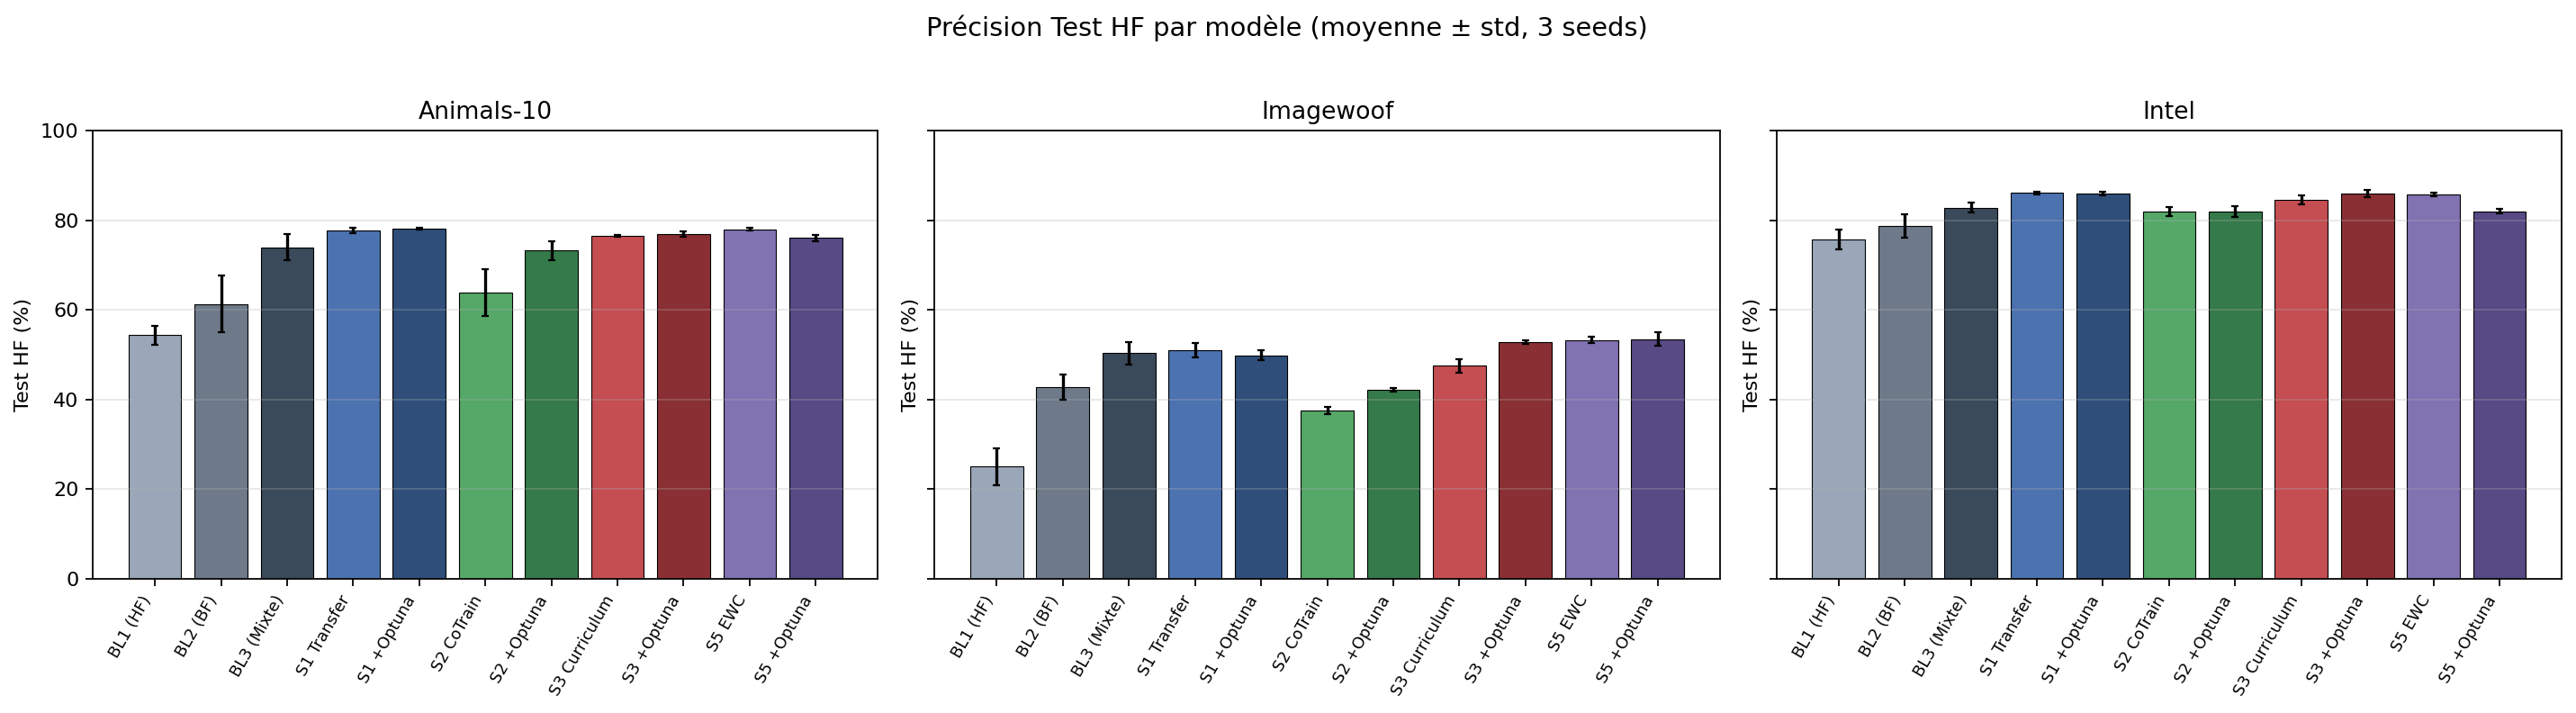
\includegraphics[width=\linewidth, height=6.9cm, keepaspectratio]{figures/hf_par_modele.png}

  \vspace{0.35em}
  {\scriptsize\color{muted} Légende des figures : « S5 » $=$ EWC $=$ Stratégie 4 ; « S3 » $=$ Curriculum $=$ Stratégie 3.}
\end{frame}

% -------------------- RÉSULTATS : PARETO --------------------
\begin{frame}{Résultats — le compromis coût / performance}
  \centering
  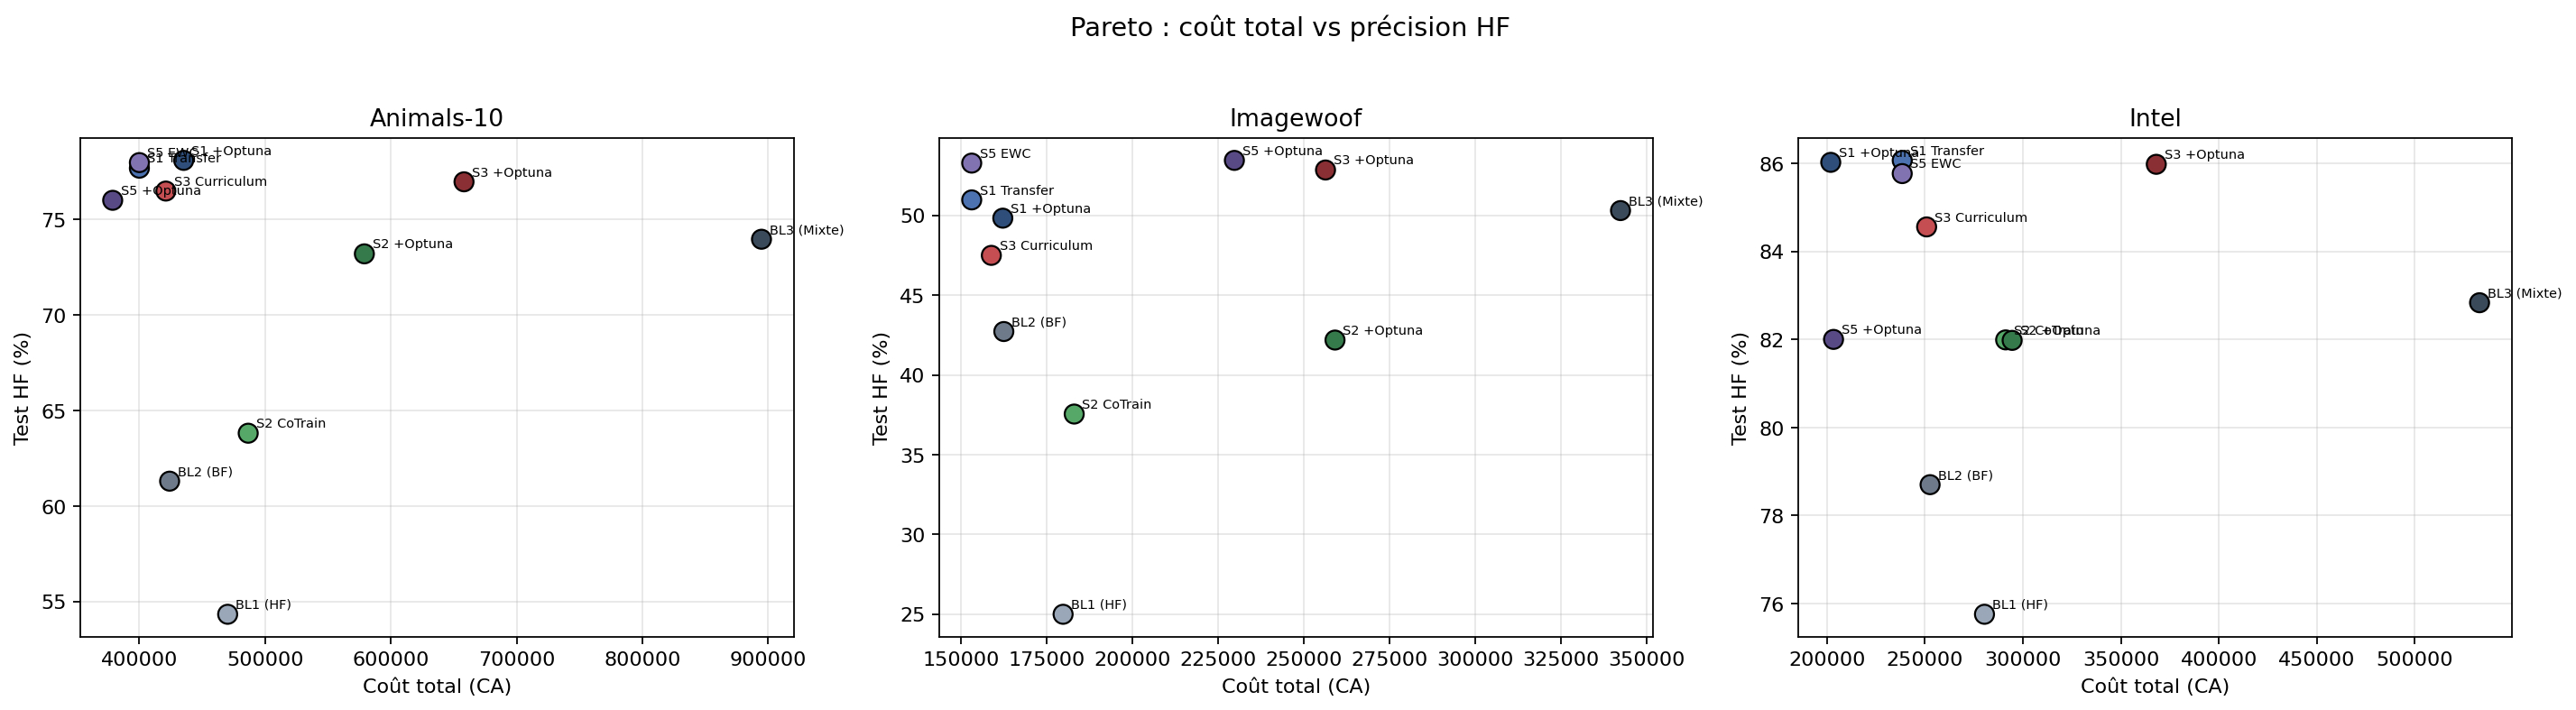
\includegraphics[width=\linewidth, height=6.5cm, keepaspectratio]{figures/pareto_cout_hf.png}

  \vspace{0.35em}
  {\scriptsize Les stratégies forment la \textbf{frontière efficiente} : on \textbf{dépasse} la borne haute (BL\,3) sur HF tout en \textbf{divisant le coût total par $\approx$2} (Animals : 400\,230 vs 894\,660 CA, à coût \emph{donnée} identique).}
\end{frame}


% -------------------- ROBUSTESSE À LA DÉGRADATION --------------------
\begin{frame}{Robustesse à la dégradation}
  \begin{columns}[c]
    \begin{column}{0.40\textwidth}
      \footnotesize
      Évaluation sur des données \emph{encore plus} dégradées que l'entraînement
      (résolution $\downarrow$, bruit $\uparrow$) :
      \begin{itemize}\setlength{\itemsep}{3pt}
        \item Arbitrage \textbf{précision-propre vs robustesse}.
        \item EWC / S1 : meilleurs sur données \emph{propres}.
        \item \textbf{Curriculum : le plus robuste} sous forte dégradation.
        \item BL\,2 (BF) : robuste à la perte de résolution, mais fragile au bruit fort.
      \end{itemize}
    \end{column}
    \begin{column}{0.58\textwidth}
      \centering
      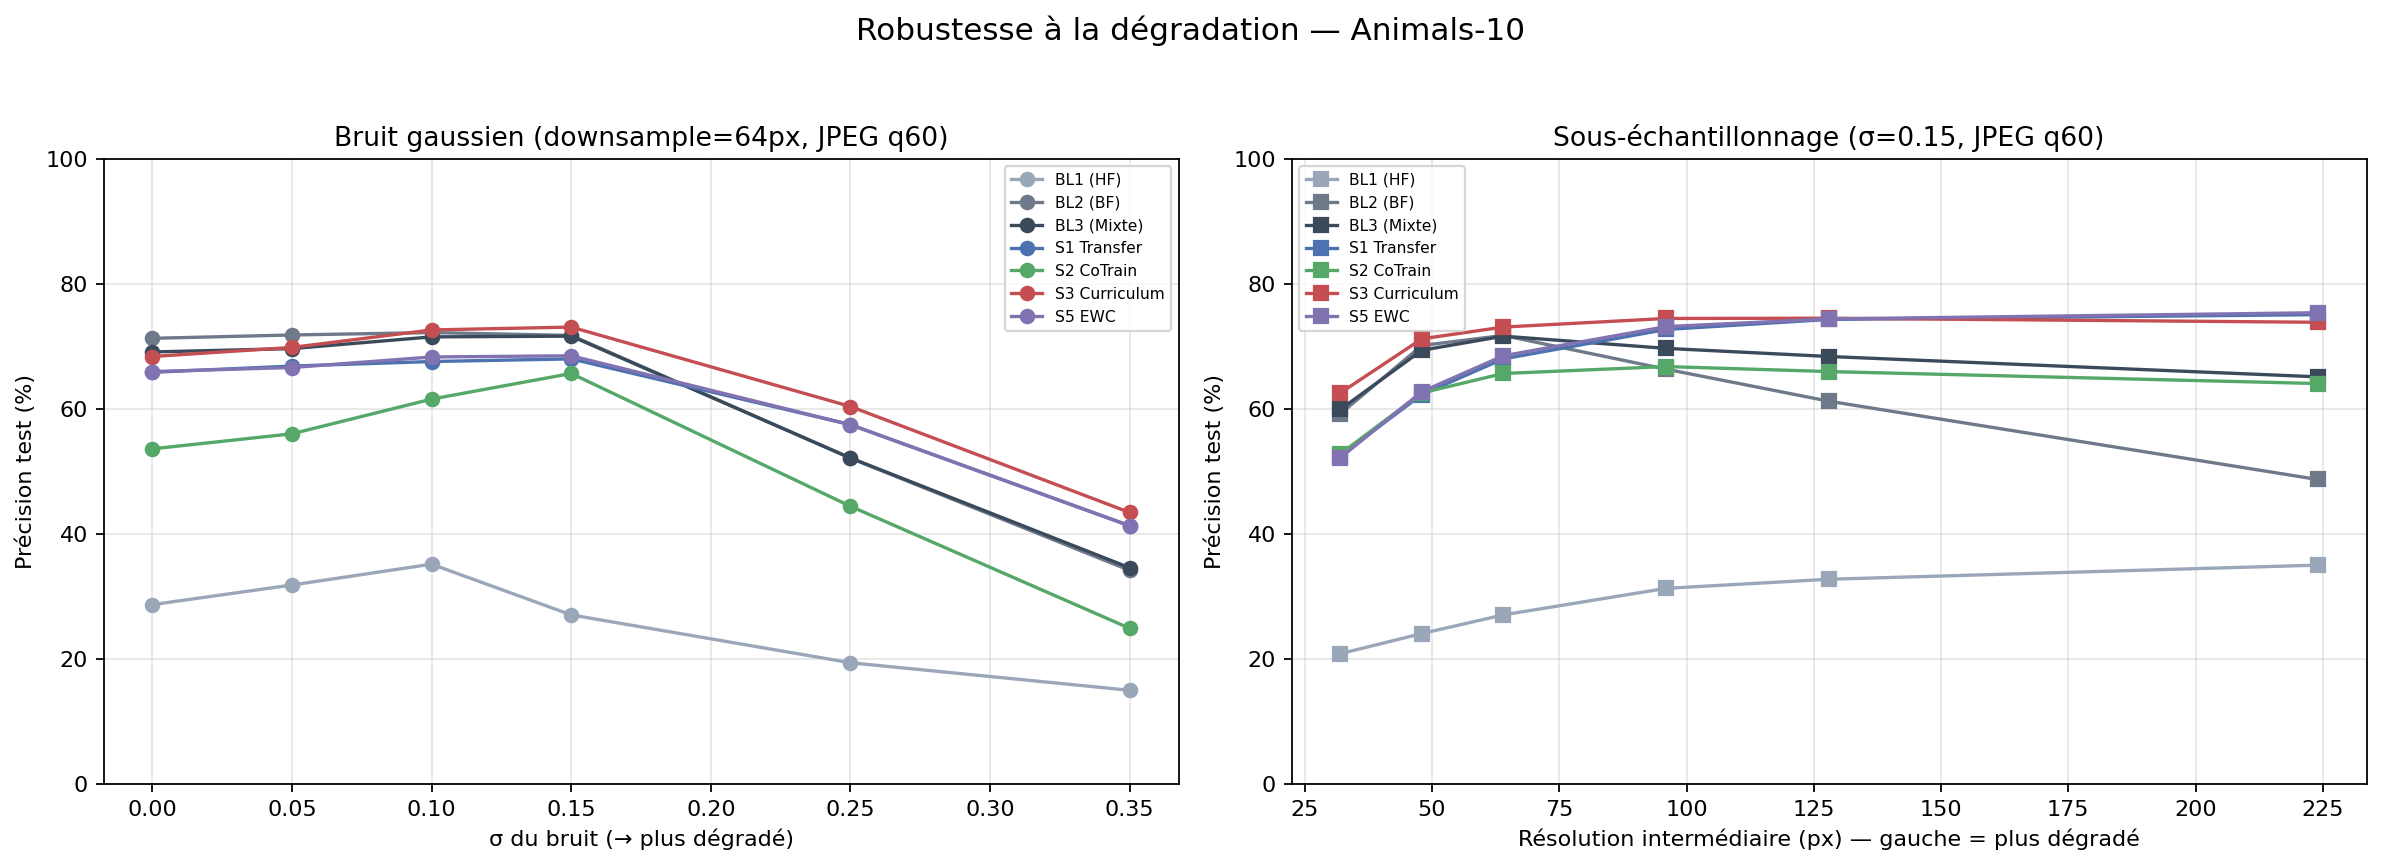
\includegraphics[width=\linewidth, height=5.0cm, keepaspectratio]{figures/robustness_degradation_animals10.png}\\[2pt]
      {\scriptsize\color{muted} Exemple Animals-10 — résolution (gauche), bruit (droite). « S5 » $=$ EWC, « S3 » $=$ Curriculum.}
    \end{column}
  \end{columns}
  \vspace{0.3em}
  \begin{key}
    \small La supériorité des stratégies multi-fidélité en \textbf{précision HF} est confirmée
    sous \textbf{multi-graines} et sur les \textbf{3 datasets}.
  \end{key}
\end{frame}

% -------------------- CONCLUSION --------------------
\begin{frame}{Conclusion \& perspectives}
  \begin{center}
    \begin{tcolorbox}[enhanced, colback=headerbg, colframe=utbmblue, boxrule=0.6pt,
      arc=2pt, width=0.92\linewidth, left=8pt, right=8pt, top=5pt, bottom=5pt]
      \centering\small
      \textbf{EWC \;$\gtrsim$\; Transfer Learning \;$>$\; Curriculum \;$>$\; Co-training
      \;$\ggg$\; baselines}
    \end{tcolorbox}
  \end{center}
  \vspace{0.2em}
  \begin{columns}[T]
    \begin{column}{0.5\textwidth}
      \textbf{À retenir}
      \begin{itemize}
        \item Objectif \textbf{atteint} : on dépasse le mélange naïf coûteux
        \textbf{à moitié prix}.
        \item \emph{Domain shift} et \emph{paradoxe de la quantité} confirmés.
        \item Résultats \textbf{cohérents} sur 3 datasets, multi-graines.
      \end{itemize}
    \end{column}
    \begin{column}{0.5\textwidth}
      \textbf{Perspectives}
      \begin{itemize}
        \item Optuna \textbf{multi-objectif} (précision \emph{et} coût).
        \item Autres \textbf{architectures} de réseau (ResNet-34, EfficientNet…).
        \item \textbf{Élargissements} : plus de datasets, de stratégies, de niveaux de fidélité, plus d'époques et d'essais Optuna.
      \end{itemize}
    \end{column}
  \end{columns}
  \vspace{0.3em}
  \begin{center}\small\color{utbmdark}
    \textbf{Des données bon marché et imparfaites : non pas un pis-aller, mais un véritable levier.}
  \end{center}
\end{frame}

% -------------------- MERCI --------------------
\begin{frame}[plain]
  \centering
  \vspace{1.0cm}
  
\includegraphics[width=3.4cm]{figures/utbm.png}\\[0.7cm]
  {\color{utbmblue}\rule{0.5\paperwidth}{1.4pt}}\\[0.4em]
  {\LARGE\bfseries\color{ink}Merci de votre attention}\\[0.3em]
  {\large\color{utbmdark}Questions \& discussion}\\[0.5em]
  {\color{utbmblue}\rule{0.5\paperwidth}{1.4pt}}\\[0.8cm]
  {\small\color{muted}Ivann Vasic \quad\textbullet\quad Module PF22 — UTBM \quad\textbullet\quad 26 juin 2026}
\end{frame}

\end{document}
